\subsubsection{Mockups}
Um die Entwicklung der App zu erleichtern, wurde als erstes ein Mockup mithilfe Figma erstellt. Figma ist eine webbasierte Vektor Grafik Softwareapplikation zur schnellen Erstellung von grafischen Oberflächen. Figma hat ausgezeichnete Cloud Integration und ermöglicht daher sehr einfache Zusammenarbeit innerhalb eines Teams. Innerhalb eines geteilten Workspace wurden erste Entwürfe für die fünf verschiedenen Menüs der Applikation erstellt.

\begin{figure}[h]
  \centering
  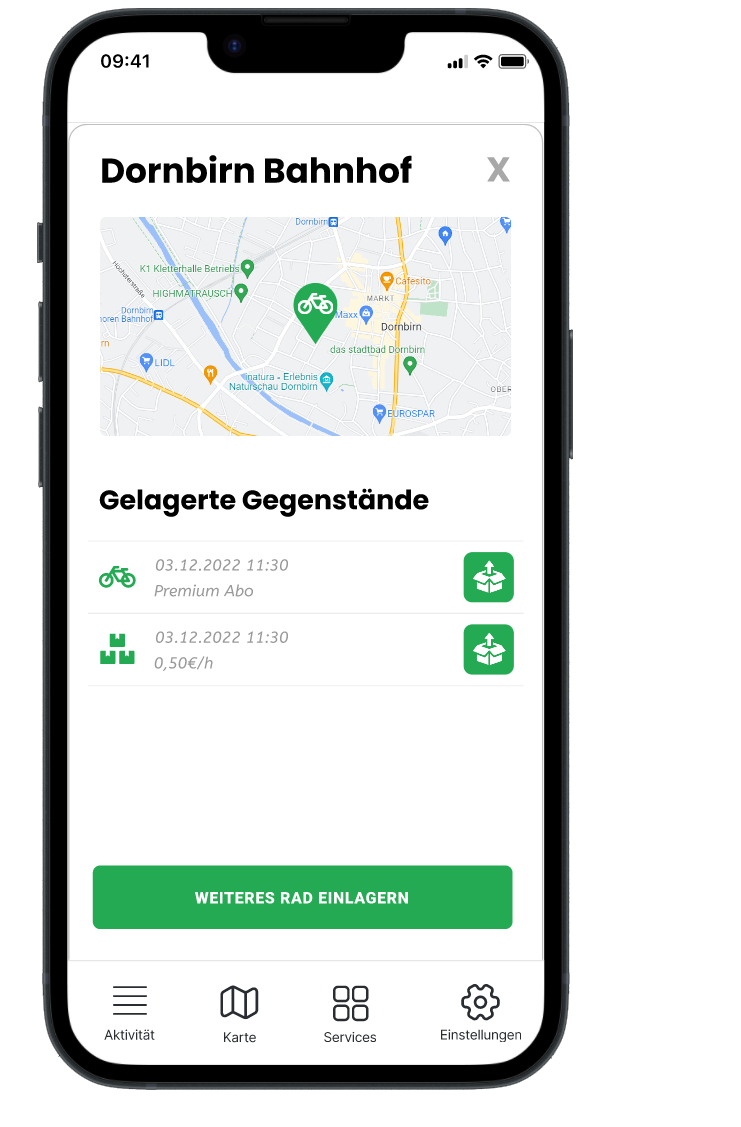
\includegraphics[width=0.15\textwidth]{images/app_mock_tower}
  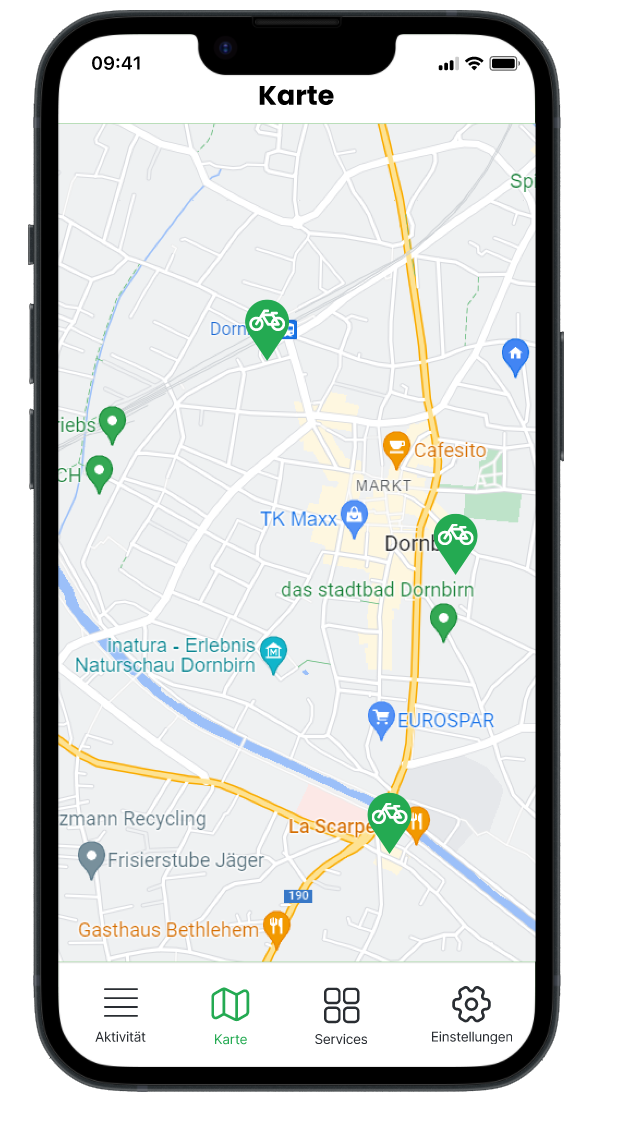
\includegraphics[width=0.15\textwidth]{images/app_mock_map}
  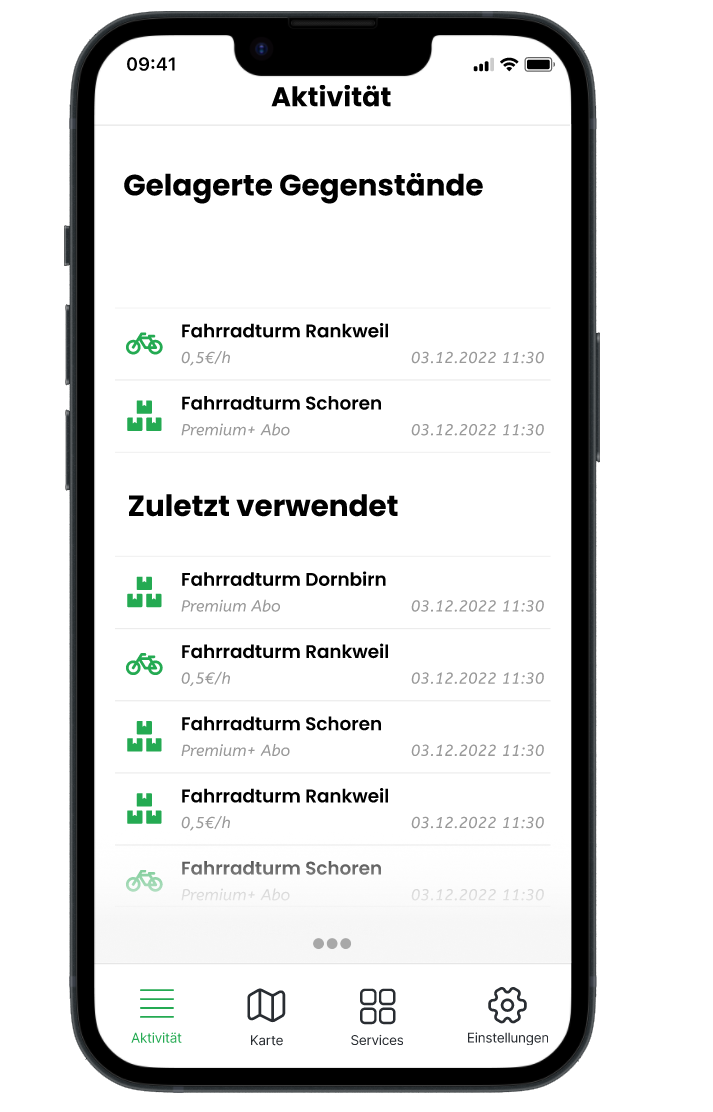
\includegraphics[width=0.15\textwidth]{images/app_mock_objects}
  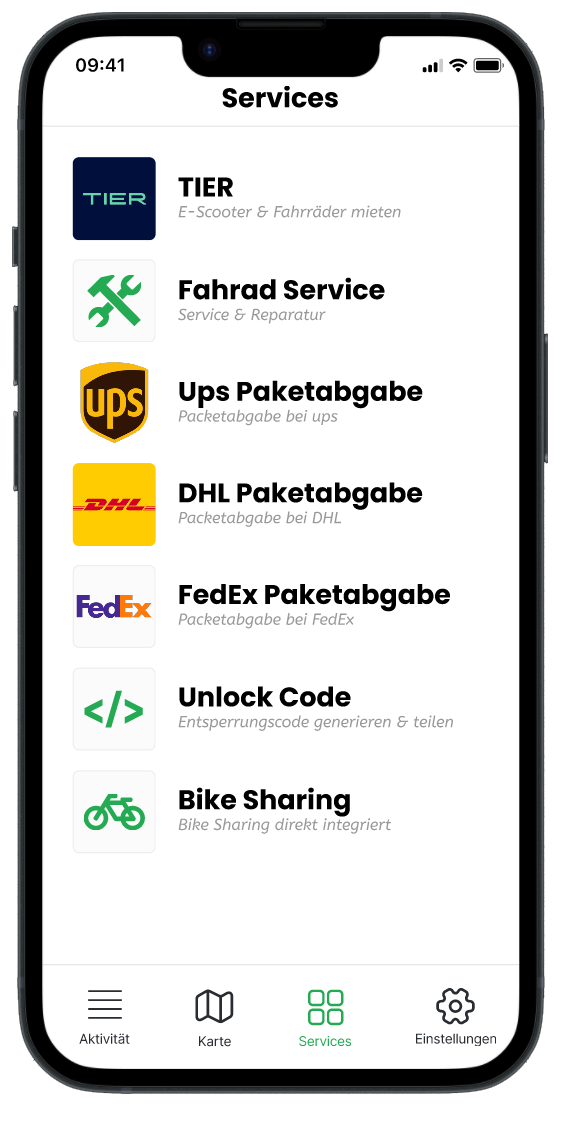
\includegraphics[width=0.15\textwidth]{images/app_mock_services}
  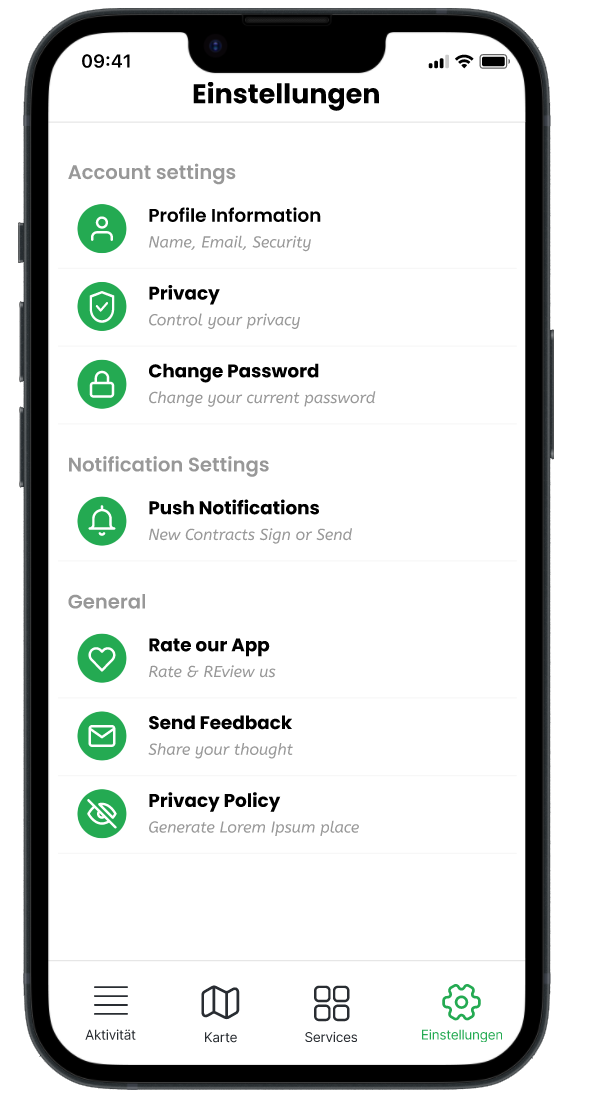
\includegraphics[width=0.15\textwidth]{images/app_mock_settings}
  \caption{App Mockup}
  \label{fig:app_mockup}
\end{figure}